\section{非光滑目标与最优条件}
\label{sec:opt-ns-optimality}

光滑目标的最优条件是梯度为零；它依赖每一点都有一条切线。本节先看尖点处还能保留哪些斜率信息：对凸目标，保留的是所有全域有效的支撑直线，由此得到次梯度、次微分以及“零属于次微分”的全局最优判据。随后计算常见目标的次微分，并整理求和与复合规则。最后作为补充说明，失去凸性后只能退回局部斜率集合，它给出的只是必要条件。

本节沿用第~\ref{chap:optimization}章的扩展实值写法：目标$f:\mathbb R^d\to\mathbb R\cup\{+\infty\}$，有效定义域$\operatorname{dom}f=\{\bm x:f(\bm x)<+\infty\}$；$f$称为适当的，是指它不取$-\infty$且$\operatorname{dom}f$非空。约束$\bm x\in C$可以写成加上指示函数$\iota_C$，它在$C$上取$0$、在$C$外取$+\infty$。

\subsection{凸次梯度与次微分}
\label{sec:opt-ns-subgradient-def}

先看最简单的尖点$f(x)=|x|$。在$x=0$右侧，函数沿斜率$1$上升；在左侧，沿斜率$-1$上升。一条直线无法同时匹配两侧，所以经典导数不存在。但第~\ref{chap:optimization}章已经说明，可微凸函数的切线总在图像下方：
\[
 f(\bm y)\geq f(\bm x)+\langle\nabla f(\bm x),\bm y-\bm x\rangle\quad\text{对所有}\ \bm y.
\]
在$|x|$的原点，切线不存在，“处处在图像下方并在当前点接触”的直线却有一整族：$y=gx$只要$-1\leq g\leq1$就满足$|y|\geq gy$。图~\ref{fig:opt-ns-abs-supports}(a)画出了其中几条。把这种全域支撑作为新的斜率信息，就得到下面的定义。

\begin{definition}[次梯度与次微分]
\label{def:opt-ns-subgradient}
设$f:\mathbb R^d\to\mathbb R\cup\{+\infty\}$是适当凸函数，$\bm x\in\operatorname{dom}f$。若向量$\bm g\in\mathbb R^d$满足
\begin{equation}
 f(\bm y)\geq f(\bm x)+\langle\bm g,\bm y-\bm x\rangle\quad\text{对所有}\ \bm y\in\mathbb R^d,
 \label{eq:opt-ns-subgradient-inequality}
\end{equation}
就称$\bm g$为$f$在$\bm x$处的\term{次梯度}（subgradient）。$f$在$\bm x$处全部次梯度组成的集合称为\term{次微分}（subdifferential），记为$\partial f(\bm x)$；对$\bm x\notin\operatorname{dom}f$，约定$\partial f(\bm x)=\varnothing$。
\end{definition}

不等式~\eqref{eq:opt-ns-subgradient-inequality}要求仿射函数$\bm y\mapsto f(\bm x)+\langle\bm g,\bm y-\bm x\rangle$在整个空间位于$f$的下方，并在$\bm x$处与$f$相等。这是一个全域条件，不是只在$\bm x$附近成立的局部近似。对每个固定的$\bm y$，满足该不等式的$\bm g$构成一个闭半空间；$\partial f(\bm x)$是所有这些闭半空间的交，因此总是闭凸集，但它可能是空集，也可能含不止一个向量。

\begin{example}[绝对值的次微分]
\label{ex:opt-ns-abs-subdifferential}
对$f(x)=|x|$逐点计算。在$x=0$处，条件是$|y|\geq gy$对所有$y$成立；取$y=1$得$g\leq1$，取$y=-1$得$g\geq-1$，反过来$|g|\leq1$时$gy\leq|g||y|\leq|y|$，所以$\partial f(0)=[-1,1]$。在$x>0$处，取$y=x+s$，$|s|<x$，条件化为$x+s\geq x+gs$，即$s\geq gs$：$s>0$时得$g\leq1$，$s<0$时得$g\geq1$，所以只能$g=1$；而$g=1$确实满足$|y|\geq y$。同理$x<0$时$\partial f(x)=\{-1\}$。
\end{example}

图~\ref{fig:opt-ns-abs-supports}(b)把这个结果画成集合值映射：离开原点时，次微分是导数构成的单点；到了原点，它变成一整段竖直线段。读者应从图中看到，尖点并没有“丢失”斜率信息，而是同时保留了左右两侧之间的全部斜率。由此也要避免一种误读：$[-1,1]$中任取一个数都只是一条支撑斜率，不能称为原点处“唯一的导数”。

\begin{figure}[!htbp]
  \centering
  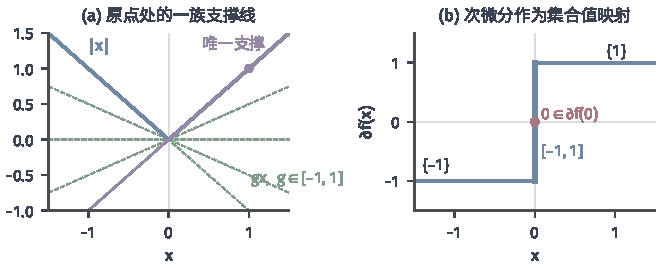
\includegraphics[width=112mm]{figures/03-optimization-evolution-and-signals/01-optimization/matplotlib/c4-abs-supports/figure.pdf}
  \caption{绝对值函数的支撑线与次微分。(a) 蓝线是$|x|$；绿色虚线是斜率$g=-1,-0.5,0,0.5,1$的直线$y=gx$，它们都在$|x|$下方并在原点接触。紫线是$x=1$处唯一的支撑线$y=x$，它与该点的切线重合。(b) 次微分$\partial|x|$：负半轴为$\{-1\}$，正半轴为$\{1\}$，原点处为竖直线段$[-1,1]$，其中含$0$（红点）。}
  \label{fig:opt-ns-abs-supports}
\end{figure}

\paragraph{可微点处的次微分}
在可微点，次微分应当回到梯度。设$f$凸，$\bm x$是$\operatorname{dom}f$的内点且$f$在$\bm x$可微。一方面，第~\ref{chap:optimization}章的一阶支撑不等式说明$\nabla f(\bm x)\in\partial f(\bm x)$。另一方面，若$\bm g\in\partial f(\bm x)$，对任意方向$\bm v$和小的$t>0$，取$\bm y=\bm x+t\bm v$得$f(\bm x+t\bm v)-f(\bm x)\geq t\langle\bm g,\bm v\rangle$；两边除以$t$并令$t\downarrow0$，得$\langle\nabla f(\bm x),\bm v\rangle\geq\langle\bm g,\bm v\rangle$。取$\bm v=\bm g-\nabla f(\bm x)$，即得$-\lVert\bm g-\nabla f(\bm x)\rVert_2^2\geq0$，所以$\bm g=\nabla f(\bm x)$。因此$\partial f(\bm x)=\{\nabla f(\bm x)\}$：次微分只在不可微处才可能多于一个元素。

\paragraph{零次梯度与全局最优}
支撑不等式最直接的用途是判定最优。若$\bm 0\in\partial f(\bm x^\star)$，把$\bm g=\bm 0$代入式~\eqref{eq:opt-ns-subgradient-inequality}就得到$f(\bm y)\geq f(\bm x^\star)$对所有$\bm y$成立；反过来，若$\bm x^\star\in\operatorname{dom}f$是全局最小点，则$f(\bm y)\geq f(\bm x^\star)+\langle\bm 0,\bm y-\bm x^\star\rangle$，即$\bm 0\in\partial f(\bm x^\star)$。

\begin{theorem}[凸目标的最优条件]
\label{thm:opt-ns-zero-subgradient}
设$f:\mathbb R^d\to\mathbb R\cup\{+\infty\}$是适当凸函数，$\bm x^\star\in\operatorname{dom}f$。则$\bm x^\star$是$f$在$\mathbb R^d$上的全局最小点，当且仅当$\bm 0\in\partial f(\bm x^\star)$。
\end{theorem}

这个判据要求的是“集合中含零”，而不是“次微分只有零”，更不是“算法这一轮取到的次梯度为零”。在$|x|$的原点，次微分是$[-1,1]$，它含零，所以原点最优；一个只返回一条支撑斜率的程序可能在原点报告$g=0.7$，这个非零读数并不否定最优性。反过来，只要某一轮确实读到了零次梯度，当前点就已被证明是全局最小点。

\paragraph{次微分可能为空}
定义域边界上可能没有任何支撑直线。取$f(x)=-\sqrt x$（$x\geq0$），在$x<0$时令$f(x)=+\infty$；它是适当凸函数。在$x=0$处，若$g$是次梯度，则对所有$y>0$有$-\sqrt y\geq gy$，即$g\leq-1/\sqrt y$；令$y\downarrow0$，右端趋于$-\infty$，不存在这样的$g$，所以$\partial f(0)=\varnothing$。图像在原点处是竖直切线，任何非竖直直线都会在原点右侧穿到图像上方。这个点不是最小点，与定理~\ref{thm:opt-ns-zero-subgradient}并不矛盾；它提醒我们，依赖“查询一条次梯度”的算法必须先确认查询点处确实能取得次梯度。在$\operatorname{dom}f$的内点处，适当凸函数的次微分总是非空的有界集，这是凸分析中的标准结论\sidecite[第23节]{rockafellar1970convex}；本章的次梯度算法例都只在这样的点上查询，例如目标在全空间取有限值的情形。

\subsection{次微分的计算}
\label{sec:opt-ns-subdifferential-calculus}

有了定义，下一步是把常见目标的次微分算出来。计算时要分清两件事：给出某一条支撑往往很容易，算法也常常只需要一条；而写出全部次微分，则需要说明没有遗漏的支撑。最优性判断用到的是后者。

\paragraph{范数与可分目标}
欧氏范数$f(\bm x)=\lVert\bm x\rVert_2$在$\bm x\neq\bm 0$处可微，梯度为$\bm x/\lVert\bm x\rVert_2$，所以$\partial f(\bm x)=\{\bm x/\lVert\bm x\rVert_2\}$。在原点，条件是$\lVert\bm y\rVert_2\geq\langle\bm g,\bm y\rangle$对所有$\bm y$成立：若$\lVert\bm g\rVert_2\leq1$，Cauchy--Schwarz不等式给出该条件；若$\lVert\bm g\rVert_2>1$，取$\bm y=\bm g$得$\lVert\bm g\rVert_2\geq\lVert\bm g\rVert_2^2$，矛盾。因此$\partial\lVert\cdot\rVert_2(\bm 0)$是闭单位球$\{\bm g:\lVert\bm g\rVert_2\leq1\}$，绝对值例中的区间$[-1,1]$是它在一维的情形。

若目标逐坐标分离，$f(\bm x)=\sum_{j=1}^df_j(x_j)$，其中每个$f_j$是一元适当凸函数，则
\begin{equation}
 \partial f(\bm x)=\partial f_1(x_1)\times\cdots\times\partial f_d(x_d).
 \label{eq:opt-ns-separable-subdifferential}
\end{equation}
右边包含于左边：把各坐标的支撑不等式相加即得。左边包含于右边：设$\bm g\in\partial f(\bm x)$，只改变第$j$个坐标、令其余坐标保持$x_i$，支撑不等式化为$f_j(y_j)\geq f_j(x_j)+g_j(y_j-x_j)$，即$g_j\in\partial f_j(x_j)$。对$\ell_1$范数$\lVert\bm x\rVert_1=\sum_j|x_j|$，这给出：$x_j\neq0$的坐标上$g_j=\operatorname{sign}(x_j)$，$x_j=0$的坐标上$g_j$可取$[-1,1]$中任意值。例如$\partial\lVert\cdot\rVert_1(2,0,-3)=\{1\}\times[-1,1]\times\{-1\}$。

\paragraph{有限仿射最大值}
设$f(\bm x)=\max_{1\leq i\leq m}\{\bm a_i^\top\bm x+b_i\}$，记在$\bm x$处取到最大值的指标集合为$I(\bm x)$，称这些分支为活跃分支。每个活跃分支都是一条支撑：对$i\in I(\bm x)$，有
\[
 f(\bm y)\geq\bm a_i^\top\bm y+b_i=f(\bm x)+\bm a_i^\top(\bm y-\bm x).
\]
次微分是凸集，所以活跃斜率的任何凸组合也是次梯度。反过来，次微分中没有别的向量。

\begin{theorem}[最大值函数的次微分]
\label{thm:opt-ns-max-subdifferential}
对$f(\bm x)=\max_{1\leq i\leq m}\{\bm a_i^\top\bm x+b_i\}$，有
\[
 \partial f(\bm x)=\operatorname{conv}\{\bm a_i:i\in I(\bm x)\},
\]
其中$\operatorname{conv}$表示\term{凸包}（convex hull），即有限个点全部凸组合构成的集合。
\end{theorem}

\begin{proof}
包含关系“$\supseteq$”已在定理前说明。为证“$\subseteq$”，设$\bm g\in\partial f(\bm x)$，记$P=\operatorname{conv}\{\bm a_i:i\in I(\bm x)\}$。$P$是有限个点的凸包，是非空紧凸集，所以连续函数$\bm a\mapsto\lVert\bm g-\bm a\rVert_2^2$在$P$上取得最小值，设最小点为$\bm p$。对任意$\bm a\in P$和$s\in(0,1]$，$\bm p+s(\bm a-\bm p)\in P$，由最小性
\[
 \lVert\bm g-\bm p\rVert_2^2\leq\lVert\bm g-\bm p-s(\bm a-\bm p)\rVert_2^2
 =\lVert\bm g-\bm p\rVert_2^2-2s\langle\bm g-\bm p,\bm a-\bm p\rangle+s^2\lVert\bm a-\bm p\rVert_2^2;
\]
消去相同项、除以$s$并令$s\downarrow0$，得$\langle\bm g-\bm p,\bm a-\bm p\rangle\leq0$。

若$\bm g\notin P$，令$\bm v=\bm g-\bm p\neq\bm 0$，则对每个$\bm a\in P$，
\[
 \langle\bm g,\bm v\rangle-\langle\bm a,\bm v\rangle
 =\langle\bm g-\bm p,\bm v\rangle+\langle\bm p-\bm a,\bm g-\bm p\rangle
 \geq\lVert\bm v\rVert_2^2>0.
\]
另一方面，非活跃分支在$\bm x$处严格小于$f(\bm x)$，由连续性，对足够小的$t>0$它们在$\bm x+t\bm v$处仍不活跃，于是
\[
 f(\bm x+t\bm v)=\max_{i\in I(\bm x)}\{\bm a_i^\top\bm x+b_i+t\bm a_i^\top\bm v\}=f(\bm x)+t\max_{i\in I(\bm x)}\bm a_i^\top\bm v.
\]
支撑不等式给出$f(\bm x+t\bm v)\geq f(\bm x)+t\langle\bm g,\bm v\rangle$，从而$\max_{i\in I(\bm x)}\bm a_i^\top\bm v\geq\langle\bm g,\bm v\rangle$，与上式矛盾。故$\bm g\in P$。
\end{proof}

证明中“紧凸集上最近点满足的内积不等式”在第~\ref{sec:opt-ns-prox-computation}小节还会对一般闭凸集系统地建立；这里只用到有限点凸包这一紧的情形。

\begin{example}[一维三段折线]
\label{ex:opt-ns-three-pieces}
取$f(x)=\max\{-x,\ x/2,\ 2x-3\}$。三条直线两两求交可知：$x\leq0$时$-x$最大，$0\leq x\leq2$时$x/2$最大，$x\geq2$时$2x-3$最大。于是在$x=0$处活跃分支为$-x$与$x/2$，$\partial f(0)=\operatorname{conv}\{-1,1/2\}=[-1,1/2]$；在$x=2$处$\partial f(2)=[1/2,2]$；其余点次微分是单个斜率。因为$0\in[-1,1/2]$，由定理~\ref{thm:opt-ns-zero-subgradient}，$x^\star=0$是全局最小点，$f^\star=0$。图~\ref{fig:opt-ns-max-affine}左图在两个切换点各画出几条支撑线，右图是$\partial f$的图像：每到一个切换点，次微分就从左侧斜率跳到右侧斜率，并在切换点处填满两者之间的整段。
\end{example}

\begin{figure}[!htbp]
  \centering
  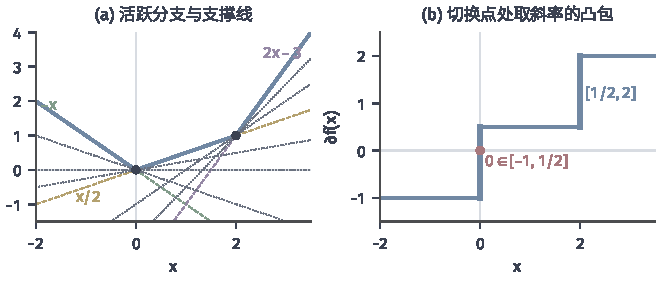
\includegraphics[width=112mm]{figures/03-optimization-evolution-and-signals/01-optimization/matplotlib/c4-max-affine-subdiff/figure.pdf}
  \caption{有限仿射最大值$f(x)=\max\{-x,x/2,2x-3\}$的次微分。(a) 蓝线是$f$，三条彩色虚线是各分支的延长线；灰色点线是切换点$x=0$与$x=2$处的几条支撑线，斜率分别取自$[-1,1/2]$与$[1/2,2]$。(b) $\partial f(x)$的图像：在切换点处取活跃斜率的凸包（竖直线段），红点标出$0\in\partial f(0)$。}
  \label{fig:opt-ns-max-affine}
\end{figure}

\paragraph{运算规则}
计算更复杂的目标，需要把次微分与加法、数乘和线性变换联系起来。对正数$\alpha>0$，支撑不等式两边同乘$\alpha$即得$\partial(\alpha f)(\bm x)=\alpha\,\partial f(\bm x)$。对仿射复合$h(\bm x)=f(\bm B\bm x+\bm c)$，若$\bm u\in\partial f(\bm B\bm x+\bm c)$，则
\[
 h(\bm y)\geq h(\bm x)+\langle\bm u,\bm B(\bm y-\bm x)\rangle=h(\bm x)+\langle\bm B^\top\bm u,\bm y-\bm x\rangle,
\]
所以$\bm B^\top\partial f(\bm B\bm x+\bm c)\subseteq\partial h(\bm x)$。同理，把两个支撑不等式相加，总有
\begin{equation}
 \partial f_1(\bm x)+\partial f_2(\bm x)\subseteq\partial(f_1+f_2)(\bm x).
 \label{eq:opt-ns-sum-inclusion}
\end{equation}

这两个包含关系的反方向都可能失败，而反方向恰恰是最优性判断需要的：若只知道$\bm 0\in\partial(f_1+f_2)(\bm x)$，却无法把它拆成两项次梯度之和，就不能写出逐项的最优条件。下面的例子说明失败确实会发生。在$\mathbb R$上取$f_1(x)=-\sqrt x$（$x\geq0$，否则为$+\infty$），$f_2=\iota_{(-\infty,0]}$。和函数只在$x=0$处有限，它就是单点集$\{0\}$的指示函数，$\partial(f_1+f_2)(0)=\mathbb R$；但前面已算出$\partial f_1(0)=\varnothing$，所以左边是空集，等式不成立。问题出在两个有效定义域只在一个边界点接触。

为了表述“定义域充分重叠”，需要相对内部的概念。$\mathbb R^d$中凸集$S$的\term{相对内部}（relative interior）$\operatorname{ri}S$，是把$S$放在它的仿射包（包含$S$的最小仿射集）中考察时的内部。例如平面中一条线段没有普通意义的内点，它的相对内部是去掉两个端点的开线段；全空间的相对内部就是全空间。

\begin{theorem}[次微分的求和与复合规则]
\label{thm:opt-ns-sum-rule}
设$f_1,f_2:\mathbb R^d\to\mathbb R\cup\{+\infty\}$是适当凸函数。若$\operatorname{ri}(\operatorname{dom}f_1)\cap\operatorname{ri}(\operatorname{dom}f_2)\neq\varnothing$，则对所有$\bm x$，
\[
 \partial(f_1+f_2)(\bm x)=\partial f_1(\bm x)+\partial f_2(\bm x).
\]
类似地，若$f$是适当凸函数且存在$\bm x_0$使$\bm B\bm x_0+\bm c\in\operatorname{ri}(\operatorname{dom}f)$，则$\partial h(\bm x)=\bm B^\top\partial f(\bm B\bm x+\bm c)$。
\end{theorem}

这两个等式的证明需要凸集分离定理，可参考前面引用的凸分析教材第23节，本章不展开。最常用的情形是其中一项在全空间取有限值：此时它的定义域是$\mathbb R^d$，相对内部条件自动成立。例如Lasso目标$\frac12\lVert\bm A\bm x-\bm b\rVert_2^2+\lambda\lVert\bm x\rVert_1$的两项都处处有限，于是
\[
 \partial\Bigl(\frac12\lVert\bm A\bm x-\bm b\rVert_2^2+\lambda\lVert\bm x\rVert_1\Bigr)
 =\bm A^\top(\bm A\bm x-\bm b)+\lambda\,\partial\lVert\bm x\rVert_1,
\]
最优条件是：$x_j\neq0$的坐标上$[\bm A^\top(\bm b-\bm A\bm x)]_j=\lambda\operatorname{sign}(x_j)$，$x_j=0$的坐标上$|[\bm A^\top(\bm b-\bm A\bm x)]_j|\leq\lambda$。一维情形$\min_x\frac12(x-3)^2+|x|$中，$x=2$满足$0\in(2-3)+\{1\}$，所以$x^\star=2$。

只有包含关系~\eqref{eq:opt-ns-sum-inclusion}时，仍然可以从“拆出的两项之和含零”推出最优，但不能反过来要求每个最小点都能这样拆分。第~\ref{sec:opt-ns-prox}节的邻近最优条件将直接用函数值比较推出，不依赖求和等式。

\subsection{非凸广义驻点（补充）}
\label{sec:opt-ns-clarke}

本小节说明失去凸性以后，尖点处的斜率信息会退化成什么；后面各节的主要结论都在凸情形下给出，跳过本小节不影响阅读。

对非凸函数，全域支撑常常不存在。$f(x)=-|x|$在原点没有任何次梯度：若$g$是次梯度，取$y=1$得$-1\geq g$，取$y=-1$得$-1\geq-g$，二者不能同时成立。可是原点处仍有清楚的局部斜率信息：两侧的导数分别是$1$和$-1$。为了保留这种信息，改为收集附近可微点上梯度的极限。

\paragraph{Clarke广义梯度}
称$f$在开集$U\subseteq\mathbb R^d$上局部Lipschitz，是指每一点都有一个邻域，在其中$|f(\bm y)-f(\bm z)|\leq K\lVert\bm y-\bm z\rVert_2$对某个常数$K$成立。这类函数在$U$中几乎处处可微，这是Rademacher定理的结论；它保证了下面的极限有足够多的可微点可取。对$\bm x\in U$，令
\[
 \partial^\circ f(\bm x)=\operatorname{conv}\Bigl\{\lim_{k\to\infty}\nabla f(\bm x_k):\bm x_k\to\bm x,\ f\text{ 在 }\bm x_k\text{ 可微，且极限存在}\Bigr\},
\]
称为\term{Clarke广义梯度}（Clarke generalized gradient）\sidecite{math-clarke1990optimization}。局部Lipschitz保证这些梯度有界，因而这是非空紧凸集。

对$|x|$与$-|x|$，原点两侧的梯度分别是$\pm1$，所以两者在原点的Clarke广义梯度都是$[-1,1]$。图~\ref{fig:opt-ns-clarke}把两种情形并排画出：两幅图中$g=0$的水平线都与这个集合相容，左图中它是全域支撑，右图中原函数却处处在它下方。同一个斜率集合，可以对应局部最小点，也可以对应局部最大点。对局部Lipschitz的凸函数，Clarke广义梯度与凸次微分一致（见前引专著第2.2节），所以它确实是次微分的推广。

\begin{figure}[!htbp]
  \centering
  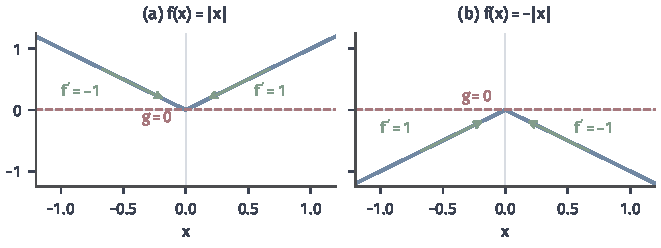
\includegraphics[width=112mm]{figures/03-optimization-evolution-and-signals/01-optimization/matplotlib/c4-clarke-abs/figure.pdf}
  \caption{同一个Clarke广义梯度对应不同的局部性质。蓝线分别是$|x|$与$-|x|$，绿色箭头标出原点两侧的导数，它们的凸包都是$[-1,1]$；红色虚线是斜率$g=0$的直线。(a) 中这条直线是全域支撑，原点是全局最小点；(b) 中原函数处处在它下方，原点是局部最大点，凸次微分为空集。}
  \label{fig:opt-ns-clarke}
\end{figure}

\paragraph{含零只是必要条件}
Clarke广义梯度有一个等价刻画：定义允许基点移动的方向导数
\[
 f^\circ(\bm x;\bm v)=\limsup_{\bm y\to\bm x,\ t\downarrow0}\frac{f(\bm y+t\bm v)-f(\bm y)}{t},
\]
则$\partial^\circ f(\bm x)=\{\bm g:\langle\bm g,\bm v\rangle\leq f^\circ(\bm x;\bm v)\ \text{对所有}\ \bm v\}$（同一专著第2.1节与第2.5节）。若$\bm x$是局部最小点，在上极限中固定$\bm y=\bm x$，对足够小的$t>0$分子$f(\bm x+t\bm v)-f(\bm x)\geq0$，所以$f^\circ(\bm x;\bm v)\geq0$对所有$\bm v$成立；由等价刻画，$\bm 0\in\partial^\circ f(\bm x)$。这说明局部极小点一定是\term{Clarke驻点}（Clarke stationary point）。

反方向不成立：$-|x|$的原点满足$0\in\partial^\circ f(0)$，却是局部最大点。凸情形中“含零”之所以能推出全局最优，靠的是全域支撑不等式；Clarke广义梯度只记录局部斜率，没有这样的不等式。因此对非凸目标，算法找到Clarke驻点只是满足了一个必要条件；要接回全局最优判据，需要额外证明目标凸，或在问题结构中找到别的证书。

\paragraph{弱凸性}
介于凸与一般非凸之间，有一类负曲率受控的函数。若存在$\rho\geq0$使$f+\frac\rho2\lVert\cdot\rVert_2^2$是凸函数，称$f$为\term{$\rho$弱凸}（$\rho$-weakly convex）。例如$\cos x$的二阶导数不小于$-1$，所以$\cos x+x^2/2$凸，$\cos x$是$1$弱凸的；$|x^2-1|$在$|x|<1$上的二阶导数为$-2$、在两个尖点处是凸的折角，所以它是$2$弱凸的。$-|x|$则不是任何$\rho$下的弱凸函数：加上光滑二次项改变不了原点处向下的折角。

对$\rho$弱凸函数，凸函数$f+\frac\rho2\lVert\cdot\rVert_2^2$的支撑不等式改写后成为
\[
 f(\bm y)\geq f(\bm x)+\langle\bm g,\bm y-\bm x\rangle-\frac\rho2\lVert\bm y-\bm x\rVert_2^2,
\]
其中$\bm g\in\partial\bigl(f+\frac\rho2\lVert\cdot\rVert_2^2\bigr)(\bm x)-\rho\bm x$：全域仿射下界换成了向下开口的二次下界。这一下界让第~\ref{sec:opt-ns-prox}节的邻近子问题在适当参数下保持可解。但弱凸并不保证驻点是全局最优：$|x^2-1|$在$x=0$处可微、导数为零，却是局部最大点。它也不是强凸性或第~\ref{chap:opt-smooth}章中梯度控制目标差的那类条件的同义词：弱凸只限制最坏的负曲率，不提供任何正曲率。
